%\documentclass[10pt,twocolumn]{article}
\documentclass[11pt]{article}

\usepackage{graphicx}% Include figure files
\usepackage{setspace}
\usepackage{dcolumn}% Align table columns on decimal point
\usepackage{bm}% bold math
\usepackage{amsmath}
\usepackage{hyperref}
\usepackage{caption}
\usepackage{listings}
\usepackage{float}
\providecommand{\e}[1]{\ensuremath{\times 10^{#1}}}

\linespread{1.0}

\begin{document}

\title{Gpvdm user manual}

\author{Roderick C. I. MacKenzie}


\maketitle




\centerline{roderick.mackenzie@nottingham.ac.uk}


\begin{figure}[ht!]
\centering
\includegraphics[width=30mm]{./images/cell.jpg}
\label{overflow}
\end{figure}

\newpage
\section{Foreword}
This manual is a work in progress, as people ask questions to do with gpvdm, I write the answer in the manual and then send the link to them.  So the text is far from exhaustive.  If something is not clear, just drop me an e-mail.  I also suggest you also read the papers which were published from this model - do also read the supplementary information (SI) to the papers, as I often write about the model in there.

\newpage

\section{Running the model}

\subsection{Installing gpvdm for windows}
Go to the download page for gpvdm at \url{http://www.gpvdm.com/windows.php} and download the latest version.  Simply double click on it and say yes to all questions.  The installer may offer you a choice of where to install the software to, don't change the install destination, the current version will only work if it is in the default install path which is C:$\backslash$gpvdm.  I publish a new exe with updates every couple of weeks, however it is possible I won't actually use gpvdm for a while after having published a new version.  Therefore, it is entirely possible that I may have introduced bugs that break the code in between releases.  So, if gpvdm is not working for, you drop me an e-mail and I will do my best to fix it asap.

\subsection{Installing gpvdm on Linux} \label{installing_on_linux}
The windows version of gpvdm seems to be much more popular than the Linux version.  Therefore, I will tend to publish an updated windows exe every couple of weeks (along with the platform independent source code) and only publish updated linux rpms/deb packages when someone asks me to.  This means that the Linux deb/rpm files tend to lag behind the windows version by about a year.  For this reason I recommend you install the Linux version from source.  If you don't want to do this, drop me an e-mail and I will often be able to push out a new rpm/deb within a day or two.  Currently I provide pre-compiled copies for, Fedora Linux, Ubuntu Linux, Debian Linux, Mint Linux , Opensuse Leap, and Raspbian pi 3.0.


\subsection{Linux from source the easy way}
Download the gpvdm by issuing the command

\begin{verbatim}
git clone  https://github.com/roderickmackenzie/gpvdm
\end{verbatim}
Find your operating system in

\begin{verbatim}
build_system/dependency_scripts
\end{verbatim}

This script should install all the packages you need to run/compile gpvdm for a given OS. I don't always keep them up to date, so if you have a new version of an OS and the packages have been renamed you may have to hunt around.

Then run:
\begin{verbatim}
./build
\end{verbatim}

Then select, (compile), and (auto). Then hit return to build.


\begin{figure}[ht!]
\centering
\includegraphics[width=120mm]{./images/build.png}
\caption{The linux build system, run ./build to get this menu.  }
\label{fig:build}
\end{figure}


\subsection{Linux from source the hard way}

On Fedora install the following pacakges:\newline
dnf install zlib-devel libzip-devel libmatheval-devel suitesparse-devel openssl-devel gsl-devel libcurl-devel blas-devel librsvg2-tools texlive ghostscript ImageMagick mencoder valgrind @development-tools fedora-packager mingw32-gcc python-crypto python-awake python3-qt5-devel python3-crypto python3-matplotlib-qt5 python3-openpyxl python3-pyopengl numpy notify-python python-inotify.noarch python-matplotlib python-inotify python-matplotlib indent unifdef indent libcurl-devel poedit ElectricFence kcachegrind help2man\newline
\newline
Then build the build system\newline
aclocal\newline
automake --add-missing\newline
automake\newline
autoconf\newline

Then configure the build system:\newline
./configure CPPFLAGS="-I/usr/include/suitesparse/"\newline

Then make the binary\newline
make\newline



\section{Running gpvdm}
On both windows and linux gpvdm will install on the start menu, click on it to launch it.  Once run, a window resembling that in figure \ref{fig:mainwindow} will appear.  From the left, the first three icons on the toolbar, open a simulation, save a simulation and generate a new simulation.  Once you have made a new simulation, the the play button will run it, and the stop button will stop the simulation running.  You will find more video examples describing how to use the model throughout the gpvdm web page.

\begin{figure}[ht!]
\centering
\includegraphics[width=140mm]{./images/main_window.png}
\caption{The main window, with a picture of the device on the right and the layer editor on the left.}
\label{fig:mainwindow}
\end{figure}


\chapter{Theory of drift diffusion modelling}
\label{sec:electrical}

\section{Outline}
Gpvdm's electrical model is a 1D/2D drift-diffusion model (like many others) however the special thing about gpvdm which makes it very good for disordered materials (Think organics, perovskites and a-Si) is that it goes to the trouble of explicitly solving the Shockley-Read-Hall equations as a function of energy and position space.  This enables one to model effects such as mobility/recombination rates changing as a function of carrier population and enables one to correctly model transients as one does not have to assume all the carriers in the trap states have reached equilibrium.  Things such as ToF transients, CELIV transients etc.. can be modelled with ease. Of course can be used for more ordered materials as well, you then just need to turn the traps off.

\section{Summary of model inputs}
A device is comprised of a series of layers (upto 10 layers), all these layers will interact with light.  Usually only one or two of these layers are electrically active, meaning the transport of electrons and holes must be modeled in detail.  Each electrically active layer with in the device has a set of electrical input parameters which define, charge transport, recombination and trapping. (see table)  If a device has more than one electrically active layer, then multiple sets of these parameters must be defined.  It should be noted that for organic materials (unlike inorganic) there is no standard set of material parameters for any given material.  The exact parameters will depend a lot on the fabrication conditions.  All layers in the device will also need a refractive index spectrum to be defined, this includes the real and imaginary refractive index as a function of wavelength (typically 300-1000 nm).
 

\section{Electrostatic potential}
The conduction band/valance band (or LUMO/HOMO in organic semiconductor speak) are defined as

\begin{equation}
E_{LUMO}=-\chi-q\phi
\end{equation}

\begin{equation}
E_{HOMO}=-\chi-E_g-q\phi
\end{equation}

To obtain the internal potential distribution within the device Poisson's equation is solved,

\begin{equation}
\label{eq:pos}
\nabla \cdot \epsilon_0 \epsilon_r \nabla = q (n_{f}+n_{t}-p_{f}-p_{t}-N_{ad}+-N_{ion}+a),
\end{equation}

where $n_{f}$, $n_{t}$ are the carrier densities of free and trapped electrons; $p_{f}$ and $p_{t}$ are the carrier densities of the free and trapped holes; and $N_{ad}$ is the doping density. $N_{ion}$ is the background density of perovskite ions and a is the density of mobile ions.

\section{Free charge carrier statistics}
For free carriers the model can either use Maxwell-Boltzmann statistics i.e.

\begin{equation}
n_{l}=N_c exp \left (\frac{F_n-E_{c}}{kT} \right)
\end{equation}

\begin{equation}
p_{l}=N_v exp \left(\frac{E_{v}-F_p}{kT} \right)
\end{equation}


or full Fermi-dirac statistics i.e.

\begin{equation}
n_{free}(E_{f},T)=\int^{\infty}_{E_{min}} \rho(E) f(E,E_{f},T) dE
\end{equation}

\begin{equation}
p_{free}(E_{f},T)=\int^{\infty}_{E_{min}} \rho(E) f(E,E_{f},T) dE
\end{equation}

where

\begin{equation}
f(E)=\frac{1}{1+e^{{E-E_f}/kT}}
\end{equation}

When using FD statistics free carriers are assumed to move in a parabolic band:

\begin{equation}
\rho(E)_{3D}=\frac{\sqrt{E}}{4\pi^2} \left ( \frac{2m^{*}}{\hbar^2}\right )^{3/2}
\end{equation}

The average energy of the carriers is defined as

\begin{equation}
\label{eq:energy}
\bar{W}(E_{f},T)=\frac{\int^{\infty}_{E_{min}} E \rho(E) f(E,E_{f},T) dE}{\int^{\infty}_{E_{min}} \rho(E) f(E,E_{f},T) dE}
\end{equation}

\section{Carrier trapping and Shockley-Read-Hall recombination}
\label{sec:SRHintro}
The model provides two methods to account for carrier trapping and recombination via trap states.  The first by equation \ref{eq:ss_srh}, this assumes that the trapped carrier distribution has reached equilibrium.  It also assumes there are relatively few trapped charge carriers compared the the number of free carriers, and thus the trapped charges do not significantly change the electrostatic potential.  These assumptions are valid when the material is very ordered (i.e. GaAs) or at a push in steady state for some moderately disordered material systems. However if you wish to simulate transient or frequency domain experiments, then you can no longer use \ref{eq:ss_srh}.  Instead, one must use a non-equilibrium SRH approach which does not assume trapped carriers have reached equilibrium.  Unlike many other models, gpvdm has such a non-equilibrium SRH model built in this is described in section \ref{sssec:dynamic}. In fact, it is turned on by default so when using gpvdm you have to go out of your way to turn on equation \ref{eq:ss_srh}.

To understand the importance of such a dynamic solver, consider the following example: You are performing a transient photocurrent experiment (TPC). You photo-excite your device with a laser, carriers very quickly become trapped during the first 1-2$\mu s$ after photoexcitation, as time passes, the carriers gradually de-trap from deeper and deeper trap states and produce the long photocurrent transient \cite{mackenzie2013interpreting}. These transients can often extend out to over 1 second after photo-excitation.  Current at the start of the transient originates from shallow traps while current at the end of the transient originates from carriers from very deep trap levels. To simulate this one has to be able to account for the gradual emptying of trap states firstly starting at the shallow traps, then progressing to deeper and deeper trap states. Were one to assume all trap states were in equilibrium one would not be able to simulate this process.

So in summary, although many others have used \ref{eq:ss_srh} to model disordered devices in time DON'T you results won't make sense. If you want to simulate anything but steady state in an ordered device turn ON the non-equilibrium solver.

\subsection{Equilibrium Shockley-Read-Hall recombination}

For some very ordered material systems where there are not many trap states it is enough to describe SRH trap states using the equation:

\begin{equation}
\label{eq:ss_srh}
R^{SRH}=\frac{np-n_{0}*p_{0}}{\tau_{p} (n+n_{1})+\tau_{n} (p+p_{1})}
\end{equation}

%/https://www.iue.tuwien.ac.at/phd/ayalew/node72.html
 where $R_{SRH}$ is the rate of SRH recombination, $n,p$ are the density of free charge carriers $n_0, p_0$, are the equilibrium density of charge carriers, $\tau_{n,p}$ are the SRH life times and $n_{1}$ and $p_{1}$ are the trapped electron and hole densities when the Fermi-level matches the trap state energy.  This can be turned on in the electrical parameter editor.

\subsection{Non-equilibrium carrier trapping and recombination using Shockley-Read-Hall trap states} \label{sssec:dynamic}


To describe charge becoming trapping into trap states and recombination associated with those states the model uses Shockley-Read-Hall (SRH) theory. A 0D depiction of this SRH recombination and trapping is shown in figure \ref{fig:dos_structure}, the free electron and hole carrier distributions are labeled as n free and p free respectively. The trapped carrier populations are denoted with n trap and p trap , they are depicted with filled red and blue boxes. SRH theory describes the rates at which electrons and holes become captured and escape from the carrier traps. If one considers a single electron trap, the change in population of this trap can be described by four carrier capture and escape rates as depicted in figure \ref{fig:dos_structure}. The rate rec describes the rate at which electrons become captured into the electron trap, $r_{ee}$ is the rate which electrons can escape from the trap back to the free electron population, $r_{hc}$ is the rate at which free holes get trapped and $r_{he}$ is the rate at which holes escape back to the free hole population. Recombination is described by holes becoming captured into electron space slice through our 1D traps. Analogous processes are also defined for the hole traps.



\begin{figure}
\includegraphics[width=40mm]{./images/dos_structure.jpg}
\caption{Trap filling in both energy and position space as the solar cell is taken from a negative bias
Carrier trapping, de-trapping, and recombination}
\label{fig:dos_structure}
\end{figure}

\begin{table}
\begin{center}
  \begin{tabular}{lll}
  \hline
  Mechanism & Symbol & Description  \\
  \hline
Electron capture rate & $r_{ec}$ & $n v_{th} \sigma_{n} N_{t}(1-f)$ \\
Electron escape rate & $r_{ee}$ & $e_{n} N_{t} f$ \\
Hole capture rate & $r_{hc}$ & $p v_{th} \sigma_{p} N_{t} f$ \\
Hole escape rate & $r_{he}$ & $e_{p} N_{t} (1-f)$\\
  \hline
\end{tabular}
\end{center}
\caption{Shockley-Read-Hall trap capture and emission rates, where $f$ is the fermi-Dirac occupation function and $N_{t}$ is the trap density of a single carrier trap.}
\label{tab:rates}
\end{table}



For each trap level the carrier balance \ref{eq:srhrate} is solved, giving each trap level an independent quasi-Fermi level. Each point in position space can be allocated between 10 and 160 independent trap states.  The rates of each process $r_{ec}$, $r_{ee}$, $r_{hc}$, and $r_{he}$ are give in table \ref{tab:rates}.

\begin{equation}
\label{eq:srhrate}
\frac{\delta n_t}{\partial t}=r_{ec}-r_{ee}-r_{hc}+r_{he}
\end{equation}

The escape probabilities are given by:

\begin{equation}
\label{eq:taile}
e_n=v_{th}\sigma_{n} N_{c} exp \left ( \frac{E_t-E_c}{kT}\right )
\end{equation}

and

\begin{equation}
\label{eq:taile}
e_p=v_{th}\sigma_{p} N_{v} exp \left ( \frac{E_v-E_t}{kT}\right )
\end{equation}

 where $\sigma_{n,p}$ are the trap cross sections, $v_{th}$ is the thermal emission velocity of the carriers, and $N_{c,v}$ are the effective density of states for free electrons or holes.  The distribution of trapped states (DoS) is defined between the mobility edges as

\begin{equation}
\label{eq:taile}
\rho^{e/h}(E)=N^{e/h}exp(E/E_{u}^{e/h})
\end{equation}

where , $N_{e/h}$ is the density of trap states at the LUMO or HOMO band edge
in states/eV and where $E_{U}^{e/h}$ is slope energy of the density of states. 

The value of $N_{t}$ for any given trap level is calculated by averaging the DoS function over the energy ($\Delta E$ ) which a trap occupies:

\begin{equation}
\label{eq:taile}
N_{t}(E)=\frac{\int^{E+\Delta E/2}_{E-\Delta E/2} \rho^{e}{E} dE}{\Delta E}
\end{equation}

The occupation function is given by the equation,
\begin{equation}
f(E_{t},F_{t})=\frac{1}{e^{\frac{E_{t}-F_{t}}{kT}}+1}
\end{equation}
Where, $E_{t}$ is the trap level, and $F_{t}$ is the Fermi-Level of the trap.
The carrier escape rates for electrons and holes are given by





\subsection{Free-to-free carrier recombination}
A free-carrier-to-free-carrier recombination (bi-molecular) pathway is also included. However, most organic solar cells have a great deal of trap states and an ideality factor greater than 1.0 suggesting that free-to-free recombination is not the dominant mechanism.  Free-to-free recombination is described using equation \ref{equ:freetofree}

\begin{equation}
R_{free}=k_{r}(n_{f}p_{f}-n_{0}p_{0})
\label{equ:freetofree}
\end{equation}

\subsection{Auger recombination}
\label{sec:auger}
Auger recombination is as

\begin{equation}
R^{AU}=(C^{AU}_{n}n+C^{AU}_{p}p)(np-n_{0}p_{0})
\end{equation}

where $C^{AU}_{n}$ and $C^{AU}_{p}$ are the Auger coefficient of electrons and holes in $m^6 s^{-1}$. This can be set in the electrical paramter editor.

%https://www.iue.tuwien.ac.at/phd/ayalew/node73.html

\section{Modelling excitons/geminate recombination - organics only}
\label{sec:dont_do_excitions}
There are a number of models to calculate the number of geminate pairs which get converted to free charge carriers the Onsager-Braun model for example will give you the exciton dissociation efficiency.  There are other models which will enable you to calculate the distribution of excitons in a device as a function of position.  However, these models will generally require a number of parameters which are often not reliably known for a material system. Such parameters include exciton life-time, diffusion length and dissociation rate. So although it's possible (and interesting) to write a model to simulate geminate recombination, one is usually better off simply introducing a \emph{photon efficiency factor} $\eta_{photon}$. This number ranges between 0.0 and 1.0 and is multiplied by the number of photons absorbed at any point in the device to account for geminate recombination losses.

\begin{equation}
\label{eq:contn}
G=G_{abs}\cdot \eta_{photon}
\end{equation}

where $G$ is the charge carrier generation rate in $m^{-3}s^{-1}$ in equations \ref{eq:contn} and  \ref{eq:contp}.
 
This factor can be obtained to a reasonable degree by comparing the difference between the simulated and experimental $J_{sc}$.  This parameter can set in the configuration section of the optical simulation window. So therefore my advice is that in most cases you should not be modelling excitons explicitly but rather using the 'photon efficiency factor'. If you really want to model excitons read on..

\subsection{Modelling excitons}
\label{sec:excitions}
So if you have read section \ref{sec:dont_do_excitions} and still think you want to model excitons this section will explain how to do it.  Gvpdm includes an exciton solver. This sits between the optical model and electrical model.  If the exciton model is turned off then generation is simply the number of photons absorbed at any point in the device multiplied by the \emph{photon efficiency factor} see equation \ref{eq:contn}. If the exciton model is turned on then optical absorption will feed straight into the exciton diffusion equation.

\begin{equation}
\label{eq:exciton}
\frac{\partial X}{\partial t} = \nabla \cdot D \nabla X +G_{optical} -k_{dis} X -k_{FRET} X- k_{PL} X-\alpha X^2.
\end{equation}

where $X$ is the exciton density as a function of position, $D$ is the diffusion constant, $G_{optical}$ exciton generation rate. This value is taken straight from the optical model.  The constant $k_{dis}$ is exciton dissociation rate to free charge carriers.  When the exciton model is switched on $G$ in equations equals $k_{dis} X$. $k_{FRET}$ is the F\"{o}ster resonance energy transfer, $k_{PL} X$ is the radiative loss and $\alpha$ is an exciton-exciton annihilation rate constant.  The diffusion term is defined as 

\begin{equation}
\label{eq:exciton}
D=\frac{L^2}{\tau}
\end{equation}

Where $L$ is exciton diffusion length and $\tau$ is the exciton lifetime.


\section{Charge carrier transport}
To describe charge carrier transport, the bi-polar drift-diffusion equations are solved in position space
for electrons,
\begin{equation}
\label{eq:ndrive}
\boldsymbol{J_n} = q \mu_e n_{f}  {\nabla E_{c}}  + q D_n  {\nabla n_{f}},
\end{equation}
and holes,
\begin{equation}
\label{eq:pdrive}
\boldsymbol{J_p} = q \mu_h p_{f}  {\nabla E_{v}}  - q D_p {\nabla p_{f}}.
\end{equation}

Conservation of charge carriers is forced by solving the charge carrier continuity equations for both electrons,
\begin{equation}
\label{eq:contn}
\nabla \boldsymbol{J_n}  = q (R-G+\frac{\partial n}{\partial t}),
\end{equation}
and holes
\begin{equation}
\label{eq:contp}
\nabla \boldsymbol{J_p} = - q (R-G+\frac{\partial p}{\partial t}).
\end{equation}

where $R$ and $G$ are the net recombination and generation rates per unit volume respectively.

\section{Perovskite mobile ion solver}
The mobile ion solver is implemented after the work of Calado \cite{calado2016evidence}

\begin{equation}
\label{eq:pdrive}
\boldsymbol{J_a} = q \mu_a a_{f}  {\nabla E_{v}}  - q D_a {\nabla a_{f}}.
\end{equation}

\begin{equation}
\label{eq:contp}
\nabla \boldsymbol{J_a} = - q \frac{\partial a}{\partial t}.
\end{equation}



\section{Semiconductor interfaces}
\subsection{Tunnelling through heterojunctions}
Tunnelling of holes through hetrojunction interfaces are is give by
\begin{equation}
\boldsymbol{J_p} = q T_{h}  ((p_{1}-p_{1}^{eq})-(p_{0}-p_{0}^{eq})),
\end{equation}

and for electrons

\begin{equation}
\boldsymbol{J_n} = -q T_{e}  ((n_{1}-n_{1}^{eq})-(n_{0}-n_{0}^{eq})).
\end{equation}

Where $T_{h}$ and $T_{e}$ represent the rate constants of the tunnelling. This can be configured in the interfaces editor.

\subsection{Doping on the interface}
Using the interface editor, layers of doping measuring one mesh point thick can be added to either side of the interface.  This is useful for OFET simulations where interface charge is important to the turn on voltage.


\newpage
\section{Configuring the electrical solver}
\label{sec:solverconfig}


Behind gpvdm are a series of non-linear solvers that solve the electrical equations in a highly efficient way.  These can be configured by going to the electrical tab. There you will see the Drift diffusion button, to the left of that is an arrow. If you click on this it will bring up a window which allows you to configure the "Newton solver". The options are described below.

Related YouTube videos:
\begin{figure}[H]

\begin{tabular}{ c l }


\includegraphics[width=0.05\textwidth]{./images/youtube.png}

&
\href{https://www.youtube.com/watch?v=D2WG1_wTbdc}{How to optimize simulations in gpvdm so they run faster}

\end{tabular}
\end{figure}

\begin{itemize}
  \item Max Electrical iterations (first step): The maximum number of steps the solver can after it's cold started onto a new problem.  This is usually at 0V in the dark.  The solver usually takes more steps on it's first go.
  \item Electrical clamp (first step): This is a number by which the maximum newton step is clamped to.  0.1 will make the solver very stable but very slow, 4.0 will make the solver very fast but unstable.  A recommended value of 1.0 is suggested for normal problems.  If you are solving for high doping or other unusual conditions it can be worth reducing the step.  Likewise if you want the solver to be fast and you know the problem is easy set the value to 2.0 or higher. For the first step, I would consider setting this value to be slightly lower than for the subsequent steps.
  \item Desired solver error (first step): This is the desired error, smaller is more accurate and slower. I would generally not accept answers above $1x10^{-5}$

  \item Max Electrical iterations: Maximum number of electrical iterations on all but the first step.
  \item Electrical clamp: Electrical clamp (first step): This is a number by which the maximum newton step is clamped to.  0.1 will make the solver very stable but very slow, 4.0 will make the solver very fast but unstable.  A recommended value of 1.0 is suggested for normal problems.  If you are solving for high doping or other unusual conditions it can be worth reducing the step.  Likewise if you want the solver to be fast and you know the problem is easy set the value to 2.0 or higher.
  \item Desired solver error: This is the desired error, smaller is more accurate and slower. I would generally not accept answers above $1x10^{-5}$

  \item Newton solver clever exit: If the solver starts bouncing in the noise then assume we can't get a better answer and quit.
  \item Newton minimum iterations: Don't allow the solver to quit before doing this number of steps.  Often the error in the first few steps of the solution can be below "Desired solver error", thus the solver can quit before finding the true answer.
  \item Solve Kirchhoff's current law in Newton solver: Solve Kirchhoff's current law in the main Newton Jacobian.

  \item Matrix solver:  This selects the matrix solver to use.
  \item Newton solver to use:
	\begin{itemize}
	  \item none: No electrical solver is selected, this is used when only solving optical or thermal problems.
	  \item newton: The standard 1D Newton solver.
	  \item newton\textunderscore 2D: The standard 2D Newton solver.
 	  \item newton\textunderscore norm: The standard 1D Newton solver but with Slotboom normalization.  This is handy when solving systems with large difference in density between minority and majority carrier density.
 	  \item poisson\textunderscore 2d: A 2D Poisson solver with no drift diffusion equations. 
	\end{itemize}
  \item Complex matrix solver:

  \item Slotboom T0: Slotboom variable for the newton\textunderscore norm solver.
  \item Slotboom D0: Slotboom variable for the newton\textunderscore norm solver.
  \item Slotboom n0: Slotboom variable for the newton\textunderscore norm solver.

  \item Use newton cache (experimental): Cache large problems to disk - experimental.
  \item Quit on convergence problem: Quit on convergence problem. Quite often 
  \item Quit on inverted Fermi-level:
  \item Solver output verbosity:

\end{itemize}

\subsection{Solver stability}
\label{sec:solverstability}

\subsubsection{Avoiding very big and very small numbers}
Try opening up MATLAB (Octave if you are on Linux) and typing in the following equation $((1e-1+1e1)-1e1)/1e-1$. Before pressing enter, try to evaluate it in your head. the $1e1$ and the $-1e1$ cancel leaving $\frac{1e-1}{1e-1}$ which equates to $1$.  Now try replacing the powers to 1 with to the 19, so type in $((1e-19+1e19)-1e19)/1e-19$, again evaluate this in your head.  Again , $1e19$ and the $-1e19$ cancel leaving $\frac{1e-19}{1e-19}$ which equates to $1$  Now let the computer evaluate the expression.  In fact this time the computer does not give you $1$ but gives you $0$. Double check that you typed it in correctly... you did so what is happening. Why is the computer giving me an answer which is 100\% wrong.  The answer is easy, computers have a limited precision. This means that they can only store a limited number of decimal places. On a modern PC it's about 15 decimal places. After this the computer starts ignoring the numbers.  So when we added $(1e-19+1e19)$ the computer could not keep track of the decimal places so it assumed that the answer was exactly $1.000000000000000e19$ and not $1.0000000000000000001e19$, then when we subtracted $-1e19$ from the answer the computer gave us zero instead of $1e-19$.  The $1e-19$ was lost in the precision.

All computers are affected by this no matter how powerful they are, this has important implications when solving device equations.  If you have too big a spread of numbers in your simulation (matrix/Jacobian) the computer won't be able to solve it easily.  So if you have very low values of mobility say $1e-19$ and very big values say $1e5$ the computer wills start to have problems solving the electrical problem. There fore generally try to reduce the spread of parameters in you model. This is important when simulating insulators.

\subsubsection{Avoid zeros}
Zeros are bad because they cause divide by zero errors. So don't have zero mobilities, carrier cross sections, tail slopes or densities of states.  It's fine to have zero recombination constants though.

\subsubsection{Very big steps in the band gap}
Big steps in the band gap will produce very small and very large carrier densities - see \emph{Avoiding very big and very small numbers} above.


\subsection{Simulating disordered devices without traps}
\emph{This section needs to be rewritten, to more generally talk about recombination and not just Langevin recombination. For a more complete view watch the video below}

Related YouTube videos:
\begin{figure}[H]

\begin{tabular}{ c l }


\includegraphics[width=0.05\textwidth]{./images/youtube.png}

&
\href{https://www.youtube.com/watch?v=2EHfulz7UDU}{Please stop simulating disordered semiconductors without trap states.}

\end{tabular}
\end{figure}


In my view Langevin recombination is in general a really bad way to describe recombination in OPV devices.  This is because the mechanism assumes Brownian motion of electrons and holes and that charge carriers of opposite polarity will recombine when they get close enough to fall into each others electrostatic field.  This picture assumes the charge carriers are free and completely neglects the influence of trap states.  I therefore think Langeving recombination should be avoided in OPVs.
But in dx.doi.org/10.1021/jp200234m you used Langevin recombination - why?: In this paper I allowed the mobility in the Langevin expression to vary as a function of carrier density i.e.
\begin{equation}
R_{free}=q k_{r}\frac{(\alpha \mu_e(n)+\beta \mu_h(n)) n_{tot} p_{tot}}{2\epsilon_0\epsilon_r}
\end{equation}

I then by defining a mobility edge and assuming any carrier below the mobility edge could not move and any carrier above it could.  I could define the averaged electron/hole mobility as: 

\begin{equation}
\mu_e(n)=\frac{\mu_e^0 n_{free}}{n_{free}+n_{trap}}
\end{equation}

and

\begin{equation}
\mu_h(n)=\frac{\mu_h^0 p_{free}}{p_{free}+p_{trap}}
\end{equation}

and if one assumes the density of free charge carriers is much smaller than the density of trapped charge carriers one can arrive at

\begin{equation}
R(n,p)=q k_{r}\frac{(\alpha \mu_e^0 n_{free} p_{trap}+\beta \mu_h p_{free} n_{trap}) }{2\epsilon_0\epsilon_r}
\end{equation}

Thus by making the mobility carrier density dependent we arrive at an expression for Langeving recombination that's dependent upon the density of free and trapped carriers (i.e. $n_{free} p_{trap}$ and $ p_{free} n_{trap}$) This is in principle the same as SRH recombination (i.e. a process involving free electrons (holes) recombining with trapped holes (electrons)).  This was a nice simple approach and it worked quite well in the steady state.  However, to make this all work I had to assume all electrons (holes) at any given position in space had a single quasi-Fermi level, which meant they were all in equilibrium with each other.  For this to be true, all electrons (holes) would have to be able to exchange energy with all other electrons (holes) at that position in space and have an infinite charge carrier thermalization velocity.  This seemed like an OK assumption in steady state when electrons (holes) had time to exchange energy, however once we start thinking about things happening in time domain, it becomes harder to justify because there are so many trap states in the device it is unlikely that charge carriers will be able to act as one equilibrated gas with one quasi-Fermi level.  On the other hand the SRH mechanism does not make this assumption, so it is probably a better description of recombination/trapping.  I would also add that I have never found a situation in OPV device modeling where SRH recombination was unable to describe the device in question.  Conclusion: SRH is better than Langevin.  




\section{Calculating the built in potential}  \label{sssec:initial}
The first step to performing a device simulation, is to calculate the built in potential of the device.  To do this we must know the following things:

\begin{itemize}

  \item The majority carrier concentrations on the contacts $n$ and $p$.
  \item The effective densities of states $N_{LUMO}$ and $N_{HOMO}$.
  \item The effective band gap $E_g$

\end{itemize}

\begin{figure}[H]
\centering
\includegraphics[width=120mm]{./images/bands.png}
\caption{Band structure of device in equilibrium.}
\label{fig:bands}
\end{figure}

\vspace{1em}
The left hand side of the device is given a reference potential of 0 V.  See figure \ref{fig:bands}.  We can then write the energy of the LUMO and HOMO on the left hand side of the device as:

\begin{equation}
E_{LUMO}=-\chi
\end{equation}

\begin{equation}
E_{HOMO}=-\chi-E_{g}
\end{equation}

For the left hand side of the device, we can use Maxwell-Boltzmann statistics to calculate the equilibrium Fermi-level ($F_i$).

\begin{equation}
p_{l}=N_v exp \left(\frac{E_{HOMO}-F_p}{kT} \right)
\end{equation}

We can then calculate the minority carrier concentration on the left hand side using $F_i$

\begin{equation}
n_{l}=N_c exp \left (\frac{F_n-E_{LUMO}}{kT} \right)
\end{equation}

The Fermi-level must be flat across the entire device because it is in equilibrium.  However we know there is a built in potential, we can therefore write the potential of the conduction and valance band on the right hand side of the device in terms of $phi$ to take account of the built in potential.

\begin{equation}
E_{LUMO}=-\chi-q\phi
\label{equ:Ev_rhs}
\end{equation}

\begin{equation}
E_{HOMO}=-\chi-E_g-q\phi
\end{equation}

we can now calculate the potential using

\begin{equation}
n_{r}=N_c exp \left (\frac{F_n-E_{LUMO}}{kT} \right)
\end{equation}
equation \ref{equ:Ev_rhs}.

The minority concentration on the right hand side can now also be calculated using.

\begin{equation}
p_{r}=N_v exp \left (\frac{E_v-F_{HOMO}}{kT} \right)
\end{equation}

The result of this calculation is that we now know the built in potential and minority carrier concentrations on both sides of the device.  Note, infinite recombination velocity on the contacts is assumed.  I have not included finite recombination velocities in the model simply because they would add four more fitting parameters and in my experience I have never needed to use them to fit any experimental data I have come across.

Once this calculation has been performed, we can estimate the potential profile between the left and right hand side of the device, using a linear approximation. From this the charge carrier densities across the device can be guessed.  The guess for potential and carrier densities, is then used to prime the main Newton solver.  Where the real value are calculated.  The Newton solver is described in the next section.



\subsection{Average free carrier mobility}
In this model there are two types of electrons (holes), free electrons (holes) and trapped electrons (holes).  Free electrons (holes) have a finite mobility of $\mu_e^0$ ($\mu_h^0$) and trapped electrons (holes) can not move at all and have a mobility of zero.  To calculate the average mobility we take the ratio of free to trapped carriers and multiply it by the free carrier mobility.:

\begin{equation}
\mu_e(n)=\frac{\mu_e^0 n_{free}}{n_{free}+n_{trap}}
\end{equation}

Thus if all carriers were free, the average mobility would be $\mu_e^0$ and if all carriers were trapped the average mobility would be 0.  It should be noted that only $\mu_e^0$ ($\mu_h^0$) are used in the model for computation and $\mu_e(n)$ is an output parameter.

The value of $\mu_e^0$ ($\mu_h^0$) is an input parameter to the model.  This can be edited in the electrical parameter editor.  The value of $\mu_e(n)$, and $\mu_h(p)$ are output parameters from the model.  The value of $\mu_e(n)$, and $\mu_h(p)$ change as a function of position, within the device, as the number of both free and trapped charge carriers change as a function of position.  The values of  $\mu_e(x)$, and $\mu_h(x)$ can be found in $mu\_n\_ft.dat$ and $mu\_p\_ft.dat$ within the $snapshots$ directory.  The spatially averaged value of mobility, as a function of time or voltage can be found in the files $dynamic\_mue.dat$ or $dynamic\_muh.dat$ within the dynamic directory.

Were one to try to measure mobility using a technique such as CELIV or ToF, one would expect to get a value closer to $\mu_e(n)$ or $\mu_h(p)$ rather than closer to $\mu_e^0$ or $\mu_h^0$.  It should be noted however, that measuring mobility in disordered materials is a difficult thing to do, and one will get a different experimental value of mobility depending upon which experimental measurement method one uses, furthermore, mobility will change depending upon the charge density profile within the device, and thus upon the applied voltage and light intensity.  To better understand this, try for example doing a CELIV simulation, and plotting $\mu_e(n)$ as a function of time (Voltage).  You will see that mobility reduces as the negative voltage ramp is applied, this is because carriers are being sucked out of the device.  Then try extracting the mobility from the transient using the CELIV equation for extracting mobility.  Firstly, the CELIV equation will give you one value of mobility, which is a simplification of reality as the value really changes during the application of the voltage ramp.  Secondly, the value you get from the equation will almost certainly not match either $\mu_e^0$ or any value of $\mu_e(n)$.  This simply highlights, the difficult of measuring $a$ value of mobility for a disordered semiconductor and that really when we quote a value of mobility for a disordered material, it really only makes sense to quote a value measured under the conditions a material will be used.  For example, for a solar cell, values of $\mu_e(n)$ and $\mu_h(n)$, would be most useful to know under 1 Sun at the $P_{max}$ point on a JV curve.



\subsection{Meshing}
\subsubsection{Editing the electrical mesh/layers}
The device structure is split up into layers of different materials.  These can be configured in layer editor.  Some of these layers will have the layer type 'active'.  An 'active' layer is a layer over which the electrical model will be applied.  The electrical model needs a finite difference mesh to to be setup for it to work.  Usually, this will be take care of automatically, by gpvdm.  However, some users will want fine control over the mesh.  The electrical mesh editor is depicted in figure \ref{fig:emesh}.


The buttons marked 1D, 2D and 3D at the top of the window can be used to toggle the simulation between 1D, 2D and 3D modes.  (Note, if you want to do 2D or 3D simulations you are best off using a default 2D simulation, such as the OFET simulation.  This is because to do 2D/3D simulations, a special newton solver configuration will be needed.) The table on the left hand side is used to configure the mesh.  The sum of the mesh layer thicknesses must exactly match that of the sum of the active layers.  If this is not the case, the model will automatically rewrite the electrical mesh, to something that has the correct dimensions but may not be what the user desires.  Automatic mesh configuration can be turned off though the cog icon.  The columns thickness and mesh points, determine the thickness of the mesh layer and the number of points on the mesh layer, if there is a uniform spacing between mesh points.  The column, 'step multiply' by how much to grow each step.  In this example, the mesh spacing is increased by a factor of 0.1 each step.  The toggle button left/right, defines on which side the mesh layer is generated.  In this example there are two mesh layers, one starting on the left and one starting on the right.  The resulting mesh is plotted in the graph at the bottom of the window.  It can be seen that a non-linear mesh has been generated.

\begin{figure}[ht!]
\centering
\includegraphics[width=140mm]{./images/emesh.png}
\caption{The electrical mesh editor}
\label{fig:emesh}
\end{figure}

\begin{figure}[ht!]
\centering
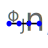
\includegraphics[width=140mm]{./images/mesh.png}
\caption{A 1D diagram of the mesh}
\label{fig:emeshdiagram}
\end{figure}


\subsubsection{Editing the optical mesh/layers}
The optical mesh automatically extends to cover the optical simulation window, so one does not usually need to worry about configuring it.  The optical material layers are defined in the list at the bottom of figure \ref{fig:emesh}.  The first column is a unique identifier, it must start with a hash symbol, but apart from that you can call it what you want.  The second column is the thickness of the layer.  The forth column is the material system, data files describing the material system are stored in the 'phys' directory.  Finally, the forth column tells the model if the layer is part of the active layer or not (more about that in the next section.)

\begin{figure}[ht!]
\centering
\includegraphics[width=140mm]{./images/opticalsimulation.png}
\caption{The electrical mesh editor}
\label{fig:opticalsimulation}
\end{figure}

\subsubsection{Interfacing the electrical and optical models}
In gpvdm there is both an electrical model and an optical model.  The optical simulation usually includes the glass substrate, the contacts and layers such as PEDOT:PSS.  The electrical simulation usually only covers the active layer of the device, thus a typically optical simulation is much bigger than the electrical simulation window.  The optical model feeds the calculated optical profile of the light into the electrical simulation.  You must therefore tell the optical model which layer in the optical simulation represents the active layer.  This is done by placing a 'yes' in the column 'Active layer' in figure \ref{fig:opticalsimulation}.
\newpage
\vfill

\subsubsection{The layer editor}
To set up and edit the vertical device structure, use the layer editor this is shown in figure \ref{fig:layer_editor}. Using this tool, you can add layers, remove layers, and move layers up and down.
\linebreak
\linebreak 
\textbf{The first column}: This is a human readable name for the layer.
\linebreak 
\linebreak 
\textbf{The second column}: The thickness of the layer in meters.
\linebreak
\linebreak 
\textbf{Third column}: Sets the optical material properties.
\linebreak
\linebreak 
\textbf{Forth column}: Sets how the model treats the layer.  The optical equations are solved over all layers.  However, if the layer is set as 'active layer', then gpvdm will the also solve the electrical equations over this layer.  More than one layer can be set as an active layer, in this case, the electrical equations will be solved over all, the layers marked 'active layer', this is useful when simulating heterojunctions.  A layer type 'other', means that the electrical equations will not be solved over that layer, but the optical equations will be.  A layer type contact, denotes that the layer represents a contact layer.  This is only affects/is needed for 2/3D simulations.


\begin{figure}[ht!]
\centering
\includegraphics[width=100mm]{./images/layer_editor.png}
{\caption{The contact editor.}}
\label{fig:layer_editor}
\end{figure}

\subsubsection{The contact editor}

The contact editor is used to edit the contacts on the device, and what voltages are applied to which contacts, see figure \ref{fig:contact_editor}.  For a 1D simulation you can pretty much ignore this window.
\linebreak
\linebreak 
\textbf{The first column}: The human readable name for the contact.
\linebreak 
\linebreak 
\textbf{The second column}: Sets if the contact is at the top or bottom of the device.  There should be at least one contact at the top and one contact at the bottom of the device.  Some devices (OFETs) can have more than one contact at the top of the device. 
\linebreak
\linebreak 
\textbf{Third column}: This sets if the contact is 'active'.  In it's simplest form, an active contact is the contact to which the voltage ramp is applied during a JV curve simulation.  In a JV curve simulation, one contact will be held at 0 volts, while a steadily increasing voltage is applied to the other 'active' contact of the device.  If you are performing a transient voltage simulation, such as CELIV, the 'active' contact will have the CELIV voltage transient applied to it.  Swapping around the active contacts is equivalent to picking up the diode and turning it through 180 degrees and placing it back in the circuit.  This feature is most useful, when simulating OFETs, when one wants to apply a voltage ramp to one contact (i.e. the gate) out of three or four.
\linebreak
\linebreak 
\textbf{Forth column}: The start of the contact, not used in 1D simulations
\linebreak
\linebreak 
\textbf{Fifth column}: The width of the contact, not used in 1D simulations.
\linebreak
\linebreak
\textbf{Sixth column}: Sets the pasavation depth under the contact. Not used in 1D simulations.
\linebreak
\linebreak  
\textbf{Seventh column}: The sets the default voltage for a contact.  If the contact type is set as 'active', this value is ignored.  However, it the contact is not active, this voltage will appear on the contact.  This use useful in OFET simulations, where you want to hold a given contact at a set voltage. 
\linebreak
\linebreak  


\begin{figure}[ht!]
\centering
\includegraphics[width=100mm]{./images/contact_editor.png}
{\caption{The contact editor.}}
\label{fig:contact_editor}
\end{figure}



\subsubsection{Scanning parameters}
Sometimes one wishes to systematically vary a simulation parameter, this is how to do it:




\begin{figure}[ht!]
\centering
\includegraphics[width=100mm]{./images/1.jpg}
{\caption*{Step 1: Select the 'Parameter scan' tool.}}
\label{overflow}
\end{figure}


\begin{figure}[ht!]
\centering
\includegraphics[width=100mm]{./images/2.jpg}
\caption*{Step 2: Add a 'scan line' to the scan.}
\end{figure}

\begin{figure}[ht!]
\centering
\includegraphics[width=100mm]{./images/3.jpg}
\caption*{Step 3: Select the new 'scan line' and the click on the 'select parameter to change' tool.}
\label{overflow}
\end{figure}


\begin{figure}[ht!]
\centering
\includegraphics[width=40mm]{./images/4.jpg}
\caption*{Step 4: Select the parameter you want to change, click apply.}
\end{figure}


\begin{figure}[ht!]
\centering
\includegraphics[width=100mm]{./images/5.jpg}
\caption*{Step 5: The 'scan line' should now be updated with the parameter you want to scan.}
\end{figure}


\begin{figure}[ht!]
\centering
\includegraphics[width=100mm]{./images/6.jpg}
\caption*{Step 6: Now enter the parameters you wish to scan, in this case 0.0-0.5 suns.
Step 7: Click the run button.}
\end{figure}


\begin{figure}[ht!]
\centering
\includegraphics[width=100mm]{./images/7.jpg}
\caption*{Step 8: Select the output file you want to plot.  gpvdm will plot all simulation results.}
\end{figure}

\subsubsection{1D, 2D and 3D simulations with gpvdm}
When deciding if you should perform 1D, 2D or 3D, simulations, consider the dimensionality of your problem.  For example if you consider a solar cell, it is only a few micros thick, and there is rapid variation in the structure, charge densities, mobilities, and doping as a function of depth (y).  However, the structure will not vary very quickly in the lateral (xz) plane.  Therefore, in general  to capture all interesting effects present within a solar cell one only needs a 1D model.  If one now considers OFETs, there is both vertical an lateral current flow, therefore one can not get away with a 1D model any more, as one must simulate both vertical current flow, and current between the source and the drain, thus one needs a 2D simulation.  As the number of dimensions increases, computation speed will decrease, therefore my general advice is to use the minimum number of dimensions possible to solve your problem.

\subsubsection{Why don't I get a 3D view of the device}
If your simulation window looks like figure \ref{fig:nothreed} and not like figure \ref{fig:threed}.  It means  either you do not have any 3D acceleration hardware on your computer, or you do not have the drivers for it installed.  If you have an ATI/Nvidia/Intel graphics card check that the drivers are installed.  Currently, not having working 3D hardware will not affect your ability to perform simulations.

\begin{figure}[ht!]
\centering
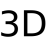
\includegraphics[width=100mm]{./images/3d.jpg}
\caption{gpvdm with working 3D acceleration hardware.}
\label{fig:threed}
\end{figure}

\begin{figure}[ht!]
\centering
\includegraphics[width=100mm]{./images/no_3d.jpg}
\caption{gpvdm with no 3D acceleration hardware.}
\label{fig:nothreed}
\end{figure}

\vfill
\clearpage


\newpage

\section{Thermal models}
\subsection{Lattice thermal model}

\subsection{Energy balance - hydrodynamic transport model}
This is an experimental feature.  From the configure window one can access the thermal simulation tab \ref{fig:thermal}, by default this model is turned off.  There are three options, the lattice thermal model which just solves the lattice heat equation; electron thermal model and hole thermal model.  The latter two solve the energy balance equations, or 3rd order moment expansion of of the Boltzmann equation.  If you turn on just the lattice model, the lattice heat equation will be solved along with the electrical model.  The thermal solver is external to the electrical solver. 

\begin{equation}
 \frac{d}{dx}\Bigg(-  \kappa_{l} \frac{dT_{L}}{dt}\Bigg)=H
\end{equation}
where H (the heat source term) is given by

\begin{equation}
H=\frac{1}{q}\frac{dE_{c}}{dx} J_{n}+\frac{1}{q}\frac{dE_{v}}{dx} J_{p}+R(E_{c}-E_{v})
\end{equation}

If you turn on the electrical and hole thermal model, then the heat source term will be replaced by

\begin{equation}
H=\frac{3 k_{b}}{2} \Bigg ( n (\frac{T_{n}-T_{l}}{\tau_{e}}) + p (\frac{T_{p}-T_{l}}{\tau_{h}})\Bigg) +R(E_{c}-E_{v})
\end{equation}

and the energy transport equation for electrons

\begin{equation}
S_n=-\kappa_n \frac{dT_{n}}{dx}-\frac{5}{2} \frac{k_{b}T_{n}}{q} J_{n}
\end{equation}

and holes,

\begin{equation}
S_p=-\kappa_p \frac{dT_{p}}{dx}+\frac{5}{2} \frac{k_{b}T_{p}}{q} J_{p}
\end{equation}

will be solved.

The energy balance equations will also be solved for electrons,

\begin{equation}
\frac{dS_{n}}{dx}=\frac{1}{q}\frac{dE_{c}}{dx} J_{n}-\frac{3 k_{b}}{2} \Bigg( R T_{n}+ n(\frac{T_{n}-T_{l}}{\tau_{e}}) \Bigg)
\end{equation}

and for holes

\begin{equation}
\frac{dS_{p}}{dx}=\frac{1}{q}\frac{dE_{v}}{dx} J_{p}-\frac{3 k_{b}}{2} \Bigg( R T_{p}+ n(\frac{T_{p}-T_{l}}{\tau_{e}}) \Bigg)
\end{equation}

The thermal conductivity of the electron gas is given by

\begin{equation}
\kappa_{n}=\Bigg ( \frac{5}{2} +c_n\Bigg) \frac{{k_{b}}^2}{q} T_{n} \mu_n n
\end{equation}

and for holes as,

\begin{equation}
\kappa_{p}=\Bigg ( \frac{5}{2} +c_p\Bigg) \frac{{k_{b}}^2}{q} T_{p} \mu_p p
\end{equation}


\begin{figure}[!htb]
\centering
\includegraphics[width=100mm]{./images/thermal.jpg}
{\caption{The thermal configuration window}}
\label{fig:thermal}
\end{figure}


\newpage

\section{Optical models}
\subsection{Ray tracing model}
\subsection{FDTD - beta}
\subsection{Transfer matrix model}
The transfer matrix model is used for simulating external light incident on the device. 
On the left of the interface the electric field is given by
\begin{equation}
E_{1}=E^{+}_{1} e^{-j k_1 z}+E^{-}_{1} e^{j k_1 z}
\label{efield1}
\end{equation}
and on the right hand side of the interface the electric field is given by
\begin{equation}
E_{2}=E^{+}_{2} e^{-j k_2 z}+E^{-}_{2} e^{j k_2 z}
\label{efield2}
\end{equation}

Maxwel's equations give us the relationship between the electric and magnetic fields for a plane wave.

\begin{equation}
\nabla \times E=-j\omega \mu H 
\end{equation}
which simplifies to:
\begin{equation}
\frac{\partial E} {\partial z}=-j\omega \mu H 
\label{maxwel}
\end{equation}

Applying equation \ref{maxwel} to equations \ref{efield1}-\ref{efield2}, we can get the magnetic field on the left of the interface
\begin{equation}
-j \mu \omega H^{y}_{1}=-j k_1 E^{+}_{1} e^{-j k_1 z}+j k_1 E^{-}_{1} e^{j k_1 z}
\end{equation}
and on the right of the interface
\begin{equation}
-j \mu \omega H^{y}_{2}=-j k_2 E^{+}_{2} e^{-j k_2 z}+j k_2 E^{-}_{2} e^{j k_2 z}.
\end{equation}

Tidying up gives,
\begin{equation}
H^{y}_{1}=\frac{k}{\omega \mu}E^{+}_{1} e^{-j k_1 z}-\frac{k}{\omega \mu} E^{-}_{1} e^{j k_1 z}
\end{equation}

\begin{equation}
H^{y}_{2}=\frac{k}{\omega \mu}E^{+}_{2} e^{-j k_2 z}-\frac{k}{\omega \mu} E^{-}_{2} e^{j k_2 z}
\end{equation}


\subsubsection{Refractive index and absorption}
\begin{equation}
E(z,t)=Re(E_0 e^{j(-kz+\omega t)})= Re(E_0 e^{j(\frac{-2 \pi (n+j\kappa)}{\lambda}z + \omega t)})=e^{\frac{2\pi\kappa z}{\lambda}}Re(E_0 e^{\frac{j(-2 \pi (n+j\kappa)}{\lambda}z +\omega t})
\end{equation}
And because the intensity is proportional to the square of the electric field the absorption coefficient becomes

\begin{equation}
e^{-\alpha x}=e^{\frac{2\pi\kappa z}{\lambda}}
\end{equation}

\begin{equation}
\alpha=-\frac{4\pi\kappa}{\lambda_0}
\end{equation}

\subsubsection{Why has the efficency of my solar cell changed now that I have upgraded to gpvdm v 4.97+}
My self and my students have recently put a lot of effort into improving the materials data base.  This means improved, absorption and refractive index data, this can affect the calculate device efficiency.  If you want to reproduce a device efficiency from a previous version of gpvdm, go to Simulations->Optica Simulation->Optical setup->Photon Efficiency. And play with this value, until you can reproduce the old efficiency.  You should only have to change the value by 20\% or so.

\subsubsection{Is Langevin recombination a good way of describing recombination OPV devices?}
In my view Langevin recombination is in general a really bad way to describe recombination in OPV devices.  This is because the mechanism assumes Brownian motion of electrons and holes and that charge carriers of opposite polarity will recombine when they get close enough to fall into each others electrostatic field.  This picture assumes the charge carriers are free and completely neglects the influence of trap states.  I therefore think Langeving recombination should be avoided in OPVs.
But in dx.doi.org/10.1021/jp200234m you used Langevin recombination - why?: In this paper I allowed the mobility in the Langevin expression to vary as a function of carrier density i.e.
\begin{equation}
R_{free}=q k_{r}\frac{(\alpha \mu_e(n)+\beta \mu_h(n)) n_{tot} p_{tot}}{2\epsilon_0\epsilon_r}
\end{equation}

I then by defining a mobility edge and assuming any carrier below the mobility edge could not move and any carrier above it could.  I could define the averaged electron/hole mobility as: 

\begin{equation}
\mu_e(n)=\frac{\mu_e^0 n_{free}}{n_{free}+n_{trap}}
\end{equation}

and

\begin{equation}
\mu_h(n)=\frac{\mu_h^0 p_{free}}{p_{free}+p_{trap}}
\end{equation}

and if one assumes the density of free charge carriers is much smaller than the density of trapped charge carriers one can arrive at

\begin{equation}
R(n,p)=q k_{r}\frac{(\alpha \mu_e^0 n_{free} p_{trap}+\beta \mu_h p_{free} n_{trap}) }{2\epsilon_0\epsilon_r}
\end{equation}

Thus by making the mobility carrier density dependent we arrive at an expression for Langeving recombination that's dependent upon the density of free and trapped carriers (i.e. $n_{free} p_{trap}$ and $ p_{free} n_{trap}$) This is in principle the same as SRH recombination (i.e. a process involving free electrons (holes) recombining with trapped holes (electrons)).  This was a nice simple approach and it worked quite well in the steady state.  However, to make this all work I had to assume all electrons (holes) at any given position in space had a single quasi-Fermi level, which meant they were all in equilibrium with each other.  For this to be true, all electrons (holes) would have to be able to exchange energy with all other electrons (holes) at that position in space and have an infinite charge carrier thermalization velocity.  This seemed like an OK assumption in steady state when electrons (holes) had time to exchange energy, however once we start thinking about things happening in time domain, it becomes harder to justify because there are so many trap states in the device it is unlikely that charge carriers will be able to act as one equilibrated gas with one quasi-Fermi level.  On the other hand the SRH mechanism does not make this assumption, so it is probably a better description of recombination/trapping.  I would also add that I have never found a situation in OPV device modeling where SRH recombination was unable to describe the device in question.  Conclusion: SRH is better than Langevin.  


\subsubsection{Should I trust the results of gpvdm?}
Yes!  The model it's self has been verified against experiment [there are over 20 publications doing this, in steady state, time domain (us-fs time scales), and fx-domain]. The basic drift-diffusion solver was cross checked and compared against other drift diffusion models, and the accuracy compared down to 6-9 dp.  While the optical model has been compared to analytical solutions of Maxwell's equations.  The SRH model has also been compared against analytical models.  If the answers you are getting out of gpvdm are odd, then I would suggest to take a look at the input parameters.  If your efficienceis are high, try increasing the number of trap states, the recombination cross sections or reducing the e/h mobilites.  Finally, I would also recommend always running the latest version, and keeping an eye on the twitter stream for bug announcements.

\section{The materials database - optical parameters}
To calculate the photondensity within the device, the model must know the refractive index and absorption of each material layer.  There are two materials databases, a read only copy and a read and writable one.  When the model starts for the first time it copies the read only materials database from C:$\backslash$Program Files$\backslash$gpvdm$\backslash$materials, to the gpvdm\_local folder in your home directory.  If you delete the copy of the materials base in the gpvdm\_local folder it will get copied back next time you start the model.  The subdirectory within the materials database identifies the material name.  In each sub directory there are two key files $alpha.omat$ and $n.omat$, these files are standard text files can be opened with any text editor such as wordpad.    Alpha.omat contains the absorption coefficient of the material while n.omat contains the the refractive index.  The first column of the file contains the wavelength in $m$ (not $cm$ or $nm$), and the second column of the file contains the absorption coefficient in $m^{-1}$ (for alpha.omat) and the real part of the refractive index (i.e. n) in au (for n.omat).

\section{The materials database - electrical parameters}
In some materials files there are also electrical parameters defined in $dos.inp$ files. These files are only used to draw the band diagrams in the optical editor..  As soon as you set a layer to be electrically active, these files will be completely ignored for that layer, with the Eg/LUMO level coming then being taken from the electrical parameters tab within the simulation window.  The only exception to this is the file $materials/generic/default/dos.inp$ which is used as the default for all newly made electrical layers.  I often get asked why I do not provide more electrical parameters with the model, as I do for the optical parameters.  The reason for this is because the proprieties of most thin film layers in devices can change by many orders of magnitude depending on how the layer is deposited (and indeed in which lab it is deposited), if you want to know the electrical parameters from your device the best way to find this is by fitting your model to experimental data.

\subsection{Adding new materials - the hard way}
If you wish to add materials to the database which do not come as standard with the model you can do it in the following way:  Simply copy an existing material directory (say C:$\backslash$Program files$\backslash$gpvdm$\backslash$materials$\backslash$ito) to a new directory (say C:$\backslash$Program files$\backslash$gpvdm$\backslash$materials$\backslash$mynewmaterial).  Then replace alpha.omat and n.omat with your data for the new material. There are two other files in each sub directory, namely fit.inp and mat.inp.  The file fit.inp is needed can be ignored, the file mat.inp is defined as follows:
\newline
\newline
\begin{lstlisting}[language=matlab,frame=single]
#LUMO		The LUMO level of the material 
4.7
#Eg		The LUMO-HOMO level of the material
0.0
#Red		Color of material in GUI
0.4
#Green		Color of material in GUI
0.4
#Blue		Color of material in GUI
0.4
#material_type	Oxide,metal,organic or inorganic.
oxide
#status		Public or private material
public
#ver		The version of the file.
1.0
#end		Defines the end of the file.
\end{lstlisting}

If you don't have data to hand for your material, but you do have a paper containing the data, you use the program Engauge Digitizer, written by  Mark Mitchell \url{https://github.com/markummitchell/engauge-digitizer} to export data from publications.  After you have finished updating the new material directory, whenever a new simulation is generated the new material files will automatically be copied into the active simulation directory ready for use. 

\subsection{Adding new materials - the easy way}
There is a youtube video on the gpvdm you tube channel describing how to do this.

\section{Changing the model}
\subsection{Editing the source code}
You can download the source code from my git hub repository \url{https://github.com/roderickmackenzie/gpvdm}.  If you do add new features yourself, please do send me patches and I will do my best to include your improvements in the main source tree.  I plan to make the source more user friendly by adding doxgen type comments, but as of yet source code comments are few and far between simply because of lack of time on my part to document.  If you have questions send me questions and I will do my best to answer.

\subsection{The structure of the model}
The model is divided into two parts, the graphical interface (GUI) and the back end solver (see \ref{fig:structureofthemodel}).  The role of the GUI, is simply to edit the input files (sim.gpvdm) and view the results.  It is the back end solver which does all the computation.  The file C:$\backslash$gpvdm$\backslash$gpvdm.exe, contains the GUI, and is a python program using a QT widget set, compiled into a windows executable.  The file C:$\backslash$gpvdm$\backslash$gpvdm\_core.exe is the back end solver which is written in C.
\begin{figure}
\centering
\includegraphics[width=100mm]{./images/architecture.png}
\caption{The structure of the model}
\label{fig:structureofthemodel}
\end{figure}
If you want to run the model from the command line, make a new simulation using the GUI, then close the GUI, and open up the terminal window.  Navigate to the directory where you saved your simulation, then enter C:$\backslash$gpvdm$\backslash$gpvdm\_core.exe in the command line.  gpvdm should then run in the terminal.

\subsection{Structure of the optical model}
I have split the optical model up into different dynamically loadable modules to so that you can write your own optical modules without too much work.  In linux these are .so files and in windows they are .dll files, these are kept in the 'light' directory.  I've not documented the interface of the plugins but if you start looking at light\_interface.c it should be pretty clear.

\subsection{Structure of the electrical solver}
I've broken the electrical model up into various plugins again to make it easier to write extra modules.  They are dynamically loaded as they are needed.  The Newton solvers and matrix inverting libraries are also plugins so they can be swapped out.


\subsection{Running gpvdm on a cluster}
Gpvdm will run on a cluster, this can be handy when doing large numbers of simulations.  To do this you need to download the cluster management code from  \url{https://github.com/roderickmackenzie/simpleclustercode}.  The clustering code as it stands is pretty much undocumented, but it should be possible to get it going.  You will have to recompile gpvdm to run on the cluster though.

\subsection{Updates}
I suggest you check the webpage regularly for updates, as I often publish minor improvements/bug fixes.  Gpvdm does have a built in update system, when it starts it connects to  \url{http://www.gpvdm.com/download_windows/update.php?ver_core=4.44&os=WinVer}, where 4.44 is replaced by your version of gpvdm and WinVer is replaced by your version of windows.  If no updates are found gpvdm.com will transmit "noupdates" back to the software.  If updates are found, the url will return the text "update 4.45" (where 4.45 is replaced with the most current verstion).  The software will then show a dialog box to inform the user that there is an update available and which version it is.    I've put this feature in, so that if I find a major bug that affects the validity of simulation results, I can inform all users quickly.  The user will then have to go and download it manually to install it.  Currently, there is no option to automatically update the software. 

\subsection{Can I use the model to simulate my exotic* material system/contacts?}
The short answer is yes.  The model is an effective medium model, meaning that it does not simulate the details of the medium, rather it approximates the medium with a set of electrical parameters.  For example, when simulating an organic solar cell, it does not simulate every detail of the BHJ, rather it just assumes an effective mobility, density of states, recombination cross sections, trapping cross sections and so on...  So if you can find electrical parameters to aproximate your material system (or guess them), there is nothing stopping you using gpvdm to simulate any exotic device/material.  The same goes for the contacts, the model simulates the contacts simply as a charge density. So if you have fancy graphene contacts which inject lots of charge, use a high majority carrier density on the contacts.  Where as if you have some dirty old ITO contacts may be drop the majority carrier density a bit.

\newpage

\section{FDTD code}
FDTD code is a new addition to gpvdm.
\begin{equation}
\frac{\partial E}{\partial t}= \frac{1}{\epsilon} \nabla \times H - \frac{1}{\epsilon} (\sigma E) 
\end{equation}


\begin{equation}
\frac{\partial E_x}{\partial t}= \frac{1}{\epsilon}(\frac{\partial H_z}{\partial y}-\frac{\partial H_y}{\partial z}-\sigma E_x) 
\end{equation}

\begin{equation}
\frac{\partial E_y}{\partial t}= \frac{1}{\epsilon}(\frac{\partial H_x}{\partial z}-\frac{\partial H_z}{\partial x}-\sigma E_y) 
\end{equation}

\begin{equation}
\frac{\partial E_z}{\partial t}= \frac{1}{\epsilon}(\frac{\partial H_y}{\partial x}-\frac{\partial H_x}{\partial y}-\sigma E_z) 
\end{equation}

Removing the z dependence because we don't care about it.

\begin{equation}
\frac{\partial E_x}{\partial t}= \frac{1}{\epsilon}(\frac{\partial H_z}{\partial y}-\sigma E_x) 
\end{equation}

\begin{equation}
\frac{\partial E_y}{\partial t}= \frac{1}{\epsilon}(-\frac{\partial H_z}{\partial x}-\sigma E_y) 
\end{equation}

\begin{equation}
\frac{\partial E_z}{\partial t}= \frac{1}{\epsilon}(\frac{\partial H_y}{\partial x}-\frac{\partial H_x}{\partial y}-\sigma E_z) 
\end{equation}


\section{Output directories}
\textbf{equilibrium}\newline
Before the solver starts any simulation it solves the device equations in the dark with 0V applied bias.  The result of this calculation are placed in this directory.  The practical reason for doing this is that Newton's method only works if you give it a reasonable starting guess for any given problem.  Thus to start the solver, we guess the carrier densities at 0V in the dark, we then use Newton's method to calculate the exact carrier density profiles at 0V in the dark (results are stored in the equilibrium directory), then from this point we can work our way to other solutions say at +1V in the light.\cite{0953-8984-25-21-215301}
\newline

\section{Output files}
Writing to disk is slow on even the most modern of computers with an SSD.  The seek speed of mechanical disks has increased little of their history.  Thus often writing the output data to the hard disk is the most time consuming part of any simulation.  By default gpvdm writes all output files to disk.  If you want to speed up your simulation, you can only write the files you need to disk.  This can be done in a fine grained way through the configure window and clicking on the detailed dump control tab.  You will from there be able to turn on and off output files.

\begin{figure}
\centering
\includegraphics[width=100mm]{./images/output_files.png}
\caption{Selecting which output files are witten to disk.}
\end{figure}

\subsubsection{1D position space output}
\paragraph{Band structure}
\textbf{Ec.dat}:LUMO-position\newline
x-axis:Position($nm$)\newline
y-axis:Electron Energy($eV$)\newline
\newline
\textbf{Efield.dat}:Material number - position\newline
x-axis:Position($nm$)\newline
y-axis:Number($au$)\newline
\newline
\textbf{Eg.dat}:Band gap-position\newline
x-axis:Position($nm$)\newline
y-axis:Electron Energy($eV$)\newline
\newline
\textbf{Ev.dat}:HOMO-position\newline
x-axis:Position($nm$)\newline
y-axis:Electron Energy($eV$)\newline
\newline
\textbf{Fi.dat}:Equlibrium Fermi-level - position\newline
x-axis:Position($nm$)\newline
y-axis:Energy($eV$)\newline
\newline
\textbf{Fn.dat}:Electron quasi Fermi-level position\newline
x-axis:Position($nm$)\newline
y-axis:Electron Energy($eV$)\newline
\newline
\textbf{Fp.dat}:Hole quasi Fermi-level position\newline
x-axis:Position($nm$)\newline
y-axis:Electron Energy($eV$)\newline
\newline
\textbf{phi.dat}:Potential\newline
x-axis:Position($nm$)\newline
y-axis:Potential($V$)\newline
\newline
\paragraph{Chaerge density}
\textbf{dn.dat}:Change in free electron population - position\newline
x-axis:Position($nm$)\newline
y-axis:Carrier density($m^{-3}$)\newline
\newline
\paragraph{Charge density}
\textbf{Nad.dat}:Doping - position\newline
x-axis:Position($nm$)\newline
y-axis:Doping density($m^{-3}$)\newline
\newline
\textbf{dnt.dat}:Excess electron density - position\newline
x-axis:Position($nm$)\newline
y-axis:Electron density($m^{-3}$)\newline
\newline
\textbf{dp.dat}:Change in free hole population - position\newline
x-axis:Position($nm$)\newline
y-axis:Carrier density($m^{-3}$)\newline
\newline
\textbf{dpt.dat}:Excess electron density - position\newline
x-axis:Position($nm$)\newline
y-axis:Hole density($m^{-3}$)\newline
\newline
\textbf{n.dat}:Total hole density - position\newline
x-axis:Position($nm$)\newline
y-axis:Carrier density($m^{-3}$)\newline
\newline
\textbf{nt.dat}:Trapped electron carrier density - position\newline
x-axis:Position($nm$)\newline
y-axis:Carrier density($m^{-3}$)\newline
\newline
\textbf{p.dat}:Total hole density - position\newline
x-axis:Position($nm$)\newline
y-axis:Carrier density($m^{-3}$)\newline
\newline
\textbf{pt.dat}:Trapped hole carrier density - position\newline
x-axis:Position($nm$)\newline
y-axis:Carrier density($m^{-3}$)\newline
\newline
\paragraph{Material parameters}
\textbf{epsilon\_r.dat}:Relative permittivity - position\newline
x-axis:Position($nm$)\newline
y-axis:Relative permittivity($au$)\newline
\newline
\textbf{mu\_n.dat}:Electron mobility - position\newline
x-axis:Position($nm$)\newline
y-axis:Electron mobility($m^{2} V^{-1} s^{-1}$)\newline
\newline
\textbf{mu\_n\_ft.dat}:Electron mobility free/all- position\newline
x-axis:Position($nm$)\newline
y-axis:Mobility($m^{2} V^{-1} s^{-1}$)\newline
\newline
\textbf{mu\_p.dat}:Hole mobility - position\newline
x-axis:Position($nm$)\newline
y-axis:Hole mobility($m^{2} V^{-1} s^{-1}$)\newline
\newline
\textbf{mu\_p\_ft.dat}:Hole mobility free/all- position\newline
x-axis:Position($nm$)\newline
y-axis:Mobility($m^{2} V^{-1} s^{-1}$)\newline
\newline
\textbf{nf.dat}:Free electron carrier density - position\newline
x-axis:Position($nm$)\newline
y-axis:Carrier density($m^{-3}$)\newline
\newline
\textbf{pf.dat}:Free hole carrier density - position\newline
x-axis:Position($nm$)\newline
y-axis:Carrier density($m^{-3}$)\newline
\newline
\paragraph{Model}
\textbf{imat.dat}:Material number - position\newline
x-axis:Position($nm$)\newline
y-axis:Number($au$)\newline
\newline
\paragraph{Recombination}
\textbf{Gn.dat}:Free electron generation rate - position\newline
x-axis:Position($nm$)\newline
y-axis:Generation rate($m^{-3} s^{-1}$)\newline
\newline
\textbf{Gp.dat}:Free hole generation rate - position\newline
x-axis:Position($nm$)\newline
y-axis:Generation rate($m^{-3} s^{-1}$)\newline
\newline
\textbf{Rn\_srh.dat}:SRH electron recombination rate - position\newline
x-axis:Position($nm$)\newline
y-axis:Recombination rate($m^{-3} s^{-1}$)\newline
\newline
\textbf{Rp\_srh.dat}:SRH hole recombination rate - position\newline
x-axis:Position($nm$)\newline
y-axis:Recombination rate($m^{-3} s^{-1}$)\newline
\newline
\textbf{R\_free.dat}:Free electron-hole recombination rate - position\newline
x-axis:Position($nm$)\newline
y-axis:Recombination rate($m^{-3} s^{-1}$)\newline
\newline
\textbf{fsrhh.dat}:Trap fermi level - position\newline
x-axis:Position($nm$)\newline
y-axis:Electron Fermi level($eV$)\newline
\newline
\textbf{fsrhn.dat}:Trap fermi level - position\newline
x-axis:Position($nm$)\newline
y-axis:Electron Fermi level($eV$)\newline
\newline
\textbf{nf\_to\_pt.dat}:Free electron to trapped hole - position\newline
x-axis:Position($nm$)\newline
y-axis:Rate($m^{-3} s^{-1}$)\newline
\newline
\textbf{nrelax.dat}:Electron relaxation rate - position\newline
x-axis:Position($nm$)\newline
y-axis:Rate($m^{-3} s^{-1}$)\newline
\newline
\textbf{pf\_to\_nt.dat}:Free hole to trapped electron - position\newline
x-axis:Position($nm$)\newline
y-axis:Rate($m^{-3} s^{-1}$)\newline
\newline
\textbf{prelax.dat}:Hole relaxation rate - position\newline
x-axis:Position($nm$)\newline
y-axis:Rate($m^{-3} s^{-1}$)\newline
\newline

\textbf{Photon\_gen.dat}:Photon generation rate - position\newline
x-axis:Position($nm$)\newline
y-axis:Photon generation rate($m^{-3} s^{-1}$)\newline

\paragraph{Transport}
\textbf{Jn.dat}:Current density - position\newline
x-axis:Position($nm$)\newline
y-axis:Electron current density($A m^{-2}$)\newline
\newline
\textbf{Jn\_diffusion.dat}:Diffusion current density - position\newline
x-axis:Position($nm$)\newline
y-axis:Electron current density (diffusion)($A m^{-2}$)\newline
\newline
\textbf{Jn\_drift.dat}:Drift current density - position\newline
x-axis:Position($nm$)\newline
y-axis:Electron current density (drift)($A m^{-2}$)\newline
\newline
\textbf{Jn\_plus\_Jp.dat}:Total current density (Jn+Jp) - position\newline
x-axis:Position($nm$)\newline
y-axis:Total current density (Jn+Jp)($A m^{-2}$)\newline
\newline
\textbf{Jp.dat}:Current density - position\newline
x-axis:Position($nm$)\newline
y-axis:Hole current density($A m^{-2}$)\newline
\newline
\textbf{Jp\_diffusion.dat}:Diffusion current density - position\newline
x-axis:Position($nm$)\newline
y-axis:Hole current density (diffusion)($A m^{-2}$)\newline
\newline
\textbf{Jp\_drift.dat}:Drift current density - position\newline
x-axis:Position($nm$)\newline
y-axis:Hole current density (drift)($A m^{-2}$)\newline
\newline
\textbf{Jp\_drift\_plus\_diffusion.dat}:Total current density (Jn+Jp) - position\newline
x-axis:Position($nm$)\newline
y-axis:Total current density (Jn+Jp)($A m^{-2}$)\newline
\newline


\textbf{sim\_info.dat}\newline
This file contains quantities calculated from the simulation such as $V_{oc}$, $J_{sc}$ what is in the file depends on what type of simulation you whish to carry out.  The file is a JSON formatted file file some common tokens are defined below:

JV curve simulation:

\begin{center}
\begin{tabular}{ |c|c|c| c|} 
\hline
JSON token & Meaning & Units & Ref \\
\hline
ff & Fill factor&au&\\
pce & 			PCE& percent&\\
Pmax & 			Power at Pmax&&\\
voc & 			$V_{oc}$ &&\\
voc\textunderscore R & 		Recombination rate at $P_{max}$& &\\
jv\textunderscore voc \textunderscore k & 		&&\\
jv\textunderscore pmax \textunderscore n & 	&&\\
voc\textunderscore nt & Trapped electron carrier densiyt at $V_oc$		&&\\
voc\textunderscore pt & Trapped hole carrier density at $V_oc$		&&\\
voc\textunderscore nf & Free electron carrier densiyt at $V_oc$		&&\\
voc\textunderscore pf & Free hole carrier density at $V_oc$		&&\\
jsc 				  & 	$J_{sc}$		& $Am^{-2}$&\\
jv\textunderscore jsc \textunderscore n & Average charge density at $J_{sc}$	& $m^{-3}$&\\
jv\textunderscore vbi & Built in voltage		& V&\\
jv\textunderscore gen & Average generation rate		&&\\
voc\textunderscore np \textunderscore tot & 	&&\\
j\textunderscore pmax & Current at $P_{max}$		& $Am^{-2}$&\\
v\textunderscore pmax & Voltage at $P_{max}$    & V &\\
mu\textunderscore jsc & 		&$m^{2} V^{-1} s^{-1}$&\\
mu\textunderscore pmax & 		&$m^{2} V^{-1} s^{-1}$&\\
mu\textunderscore voc & 	Average mobility at $V_{oc}$	& $m^{2} V^{-1} s^{-1}$&\\
mue\textunderscore pmax & Average electron mobility at $P_{max}$	&$m^{2} V^{-1} s^{-1}$&\\
muh\textunderscore pmax & Average hole mobility at $P_{max}$ &$m^{2} V^{-1} s^{-1}$&\\
tau\textunderscore voc & 	Recombination time constant at $V_{oc}$	 & s &\\
tau\textunderscore pmax & 	Recombination time constant at $P_{max}$	&s&\\

theta\textunderscore srh\textunderscore free & $\theta_{SRH}$ Collection coefficient at $P_{max}$ y & au &p.100 5.2a\cite{Summon-FETCH-bonn_catalog_45326403},\cite{PhysRevApplied.6.024001}\\
theta\textunderscore srh\textunderscore free\textunderscore trap & $\theta_{SRH}$ Collection coefficient at $P_{max}$ & au &p.100 5.2a\cite{Summon-FETCH-bonn_catalog_45326403},\cite{PhysRevApplied.6.024001}\\

\hline
\end{tabular}
\end{center}

Optical simulation

\begin{center}
\begin{tabular}{ |c|c|c| c|} 
\hline
JSON token & Meaning & Units & Ref \\
\hline
J\textunderscore photo & Photo current density $Am^{-2}$& &\\
I\textunderscore photo & Photo current $A$& &\\


\hline
\end{tabular}
\end{center}

\section{Copyright of the manual}
This manual is released under CC-BY license.

\bibliographystyle{gpvdm.bst}
\bibliography{gpvdm}



\end{document}

